\section{Geodaten}

Geodaten sind in heutigen Zeit allgegenwärtig und spielen eine zentrale Rolle in der Wirtschaft, Wissenschaft, öffentlicher Verwaltung sowie im privaten Leben. Diese Daten sind digitale Darstellung räumlicher Informationen, die einen direkten und indirekten Raumbezug zur Erdoberfläche haben. Diese Daten beschreiben Lage und Beziehungen zwischen verschiedenen Geoobjekten sowie qualitative und quantativen Merkmale dieser Objekte.\\

Geoobjekte sind räumliche Elemente, die zusätzlich zu Sachinformationen geometrische und topologische Eigenschaften besitzen und zeitlichen Veränderungen unterliegen können. Es handelt sich dabei um physische Objekte wie Gebäude, Straßen, Flüsse, Berge, Städte oder auch um abstrakte Elemente wie Verwaltungsgrenzen, Postleitzahlgebiete etc. Geoobjekte werden auf der Erdoberfläche im Form von Punkten, Linien und Polygonen dargestellt \citep{de_lange_geoinformatik_2020}.

\begin{itemize}
    \item Die \textbf{geometrische Eigenschafen} sind die Informationen zur absoluten Lage und zur Form des Objektes auf der Erdoberfläche.
    \item Die \textbf{topologischen Eigenschaften} beschreiben Umgebung bzw. Umgebungsbeziehungen, Nachbarschaften bzw. Nachbarschaftsbeziehungen, Teilmengen oder Überlagerungen. Die Geoobjekte können verschiedene Sachthemen aufweisen und zudem eine zeitliche Variabilität besitzen.
\end{itemize}

Für die Erhebung von Geodaten ist ein \textbf{Raumbezug} notwendig. D.h., dass Geoobjekten eine bestimmte Position auf der Erde und ein Verhältnis zu anderen Geoobjekten zugeordnet werden kann. Dafür wurden Modelle entwickelt, die sich der Figur der Erde möglichst genau annähern und mathematisch erfassbar sind. \\

Geodaten werden durch ihren Standort auf der Erde beschrieben. Es gibt viele Quellen für Geodaten (z. B. Fernerkundung, Punktwolkendaten, LiDAR, GPS, Internet, IoT usw.), die mit unterschiedlichen Auflösungen und Eigenschaften erfasst werden. Zwei große Kategorien sind Rasterdaten und Vektordaten. Die geografischen Merkmale auf der Erdoberfläche können in Form von Punkten, Linien und Polygonen dargestellt werden, und ihre Koordinaten werden durch Geoinformationssystem (Abschnitt. 2.5) verarbeitet und dargestellt.\\

\textbf{Vektordatenmodell} beschreibt raumbezogene Objekte anhand von Punkten, die in Form von Koordinaten definiert werden. Die Punkte werden genutzt, um Objektgeometrie zu erfassen. Ein Vektor ist nach lateinischer Übersetzung ein „Träger“ oder auch „Fahrer“ von geometrischen Informationen. \textbf{Rasterdatenmodell} stellt raumbezogene computerlesbare Geodaten mit bildhaftem Informationsgehalt dar. Die Geoinformationen werden in Pixel zerlegt. Durch die Verknüpfung von Geodaten und Sachdaten entstehen Geoinformationen, d. h. interpretierte Daten mit Raumbezug, die sich auf Orte oder Bereiche der Erdoberfläche beziehen \citep{klaus_geomatik_2023}. Abbildung 2.2 zeigt die schematische Struktur von Geodaten und unterschiedlichen Typen von Geometrie (Punkt, Linien und Polygone). Hier wird ersichtlich, wie Geodaten organisiert werden, um sowohl ihre räumliche Darstellung als auch ihre sachliche Informationen zu erfassen.\\

\begin{figure}[ht]
  \centering
  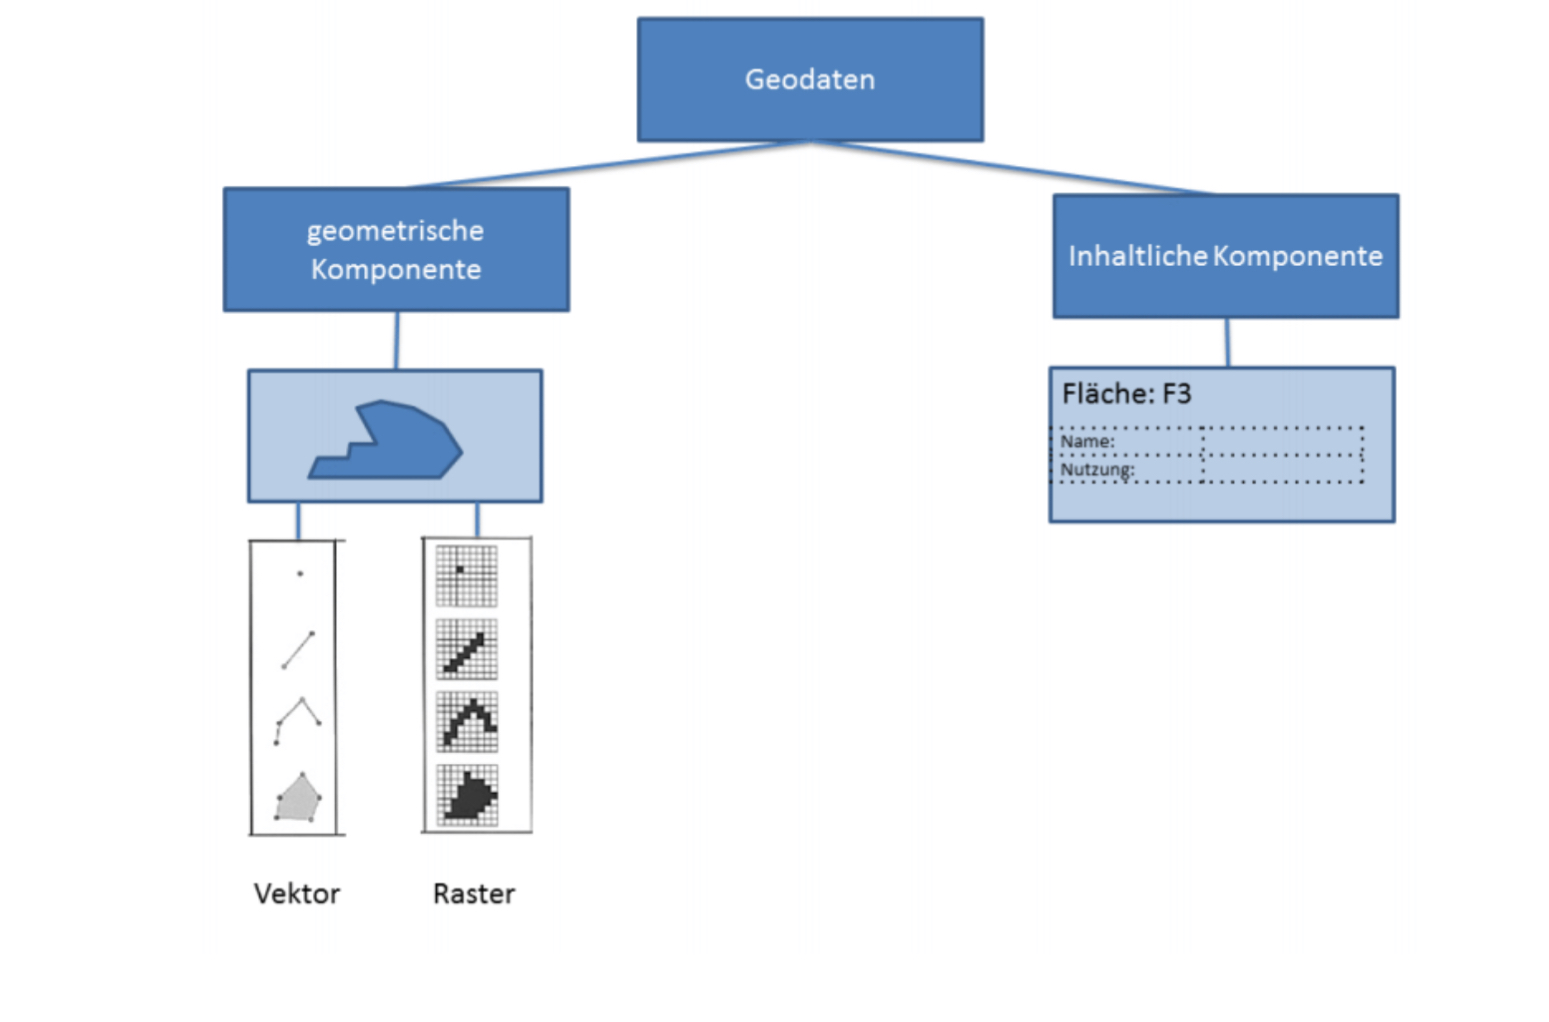
\includegraphics[width=\linewidth]{images/geodaten.jpeg}
  \caption{schematische Darstellung von Geodaten \citep{masterarbeit_fischer}}
  \label{fig:meineabbildung}
\end{figure}

...Weitere Quellen der spezifischen Geodaten\\

In diesem Projekt wird auf die Schulen in Münster, Nordrhein-Westfalen konzentriert. Die erforderlichen Geodaten für diese Schulen und ihre Umgebung sind auf der Webseite von \cite{schulen_geodaten} frei zugänglich und können uneingeschränkt genutzt werden. Die Geodaten sind Schulstandorte in NRW als Shape zum Download gestellt. Für die Speicherung der digitalen Geodaten wurden spezielle Datenbanklösungen entwickelt. Sie werden im nächsten Abschnitt vorgestellt.





% Ein \textbf{geodätisches Koordinatensystem} basiert auf einem mathematischen Model der Erde (Geoid oder Referenzellipsoid) und ermöglicht es, genaue Position (Längen- und Breitengrade) von Geoobjekten zu bestimmen. Es handelt sich dabei um ein globales Referenzsystem, das die Krümmung der Erde berücksichtigt, um präzise Lageinformationen zu liefern.

% \begin{figure}[ht]
%   \centering
%   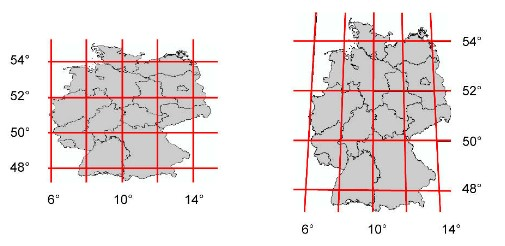
\includegraphics[width=\linewidth]{images/karte-in-deutschland.jpg}
%   \caption{Umrisse der Bundesrepublik Deutschland in einem kartesischen Koordinatensystem und in der winkeltreuen Lambert-Projektion}
%   \label{fig:meineabbildung}
% \end{figure}

% Eine \textbf{Projektion} ist eine Methode, um die dreidimensionale Oberfläche der Erde auf eine zweidimensionale Karte zu übertragen. Da es unmöglich ist, die gekrümmte Oberfläche der Erde ohne Verzerrungen auf eine flache Karte zu projizieren, gibt es verschiedene Projektionsarten, die je nach Anwendung und Region unterschiedliche Eigenschaften und Verzerrungen aufweisen.

% \begin{figure}[ht]
%   \centering
%   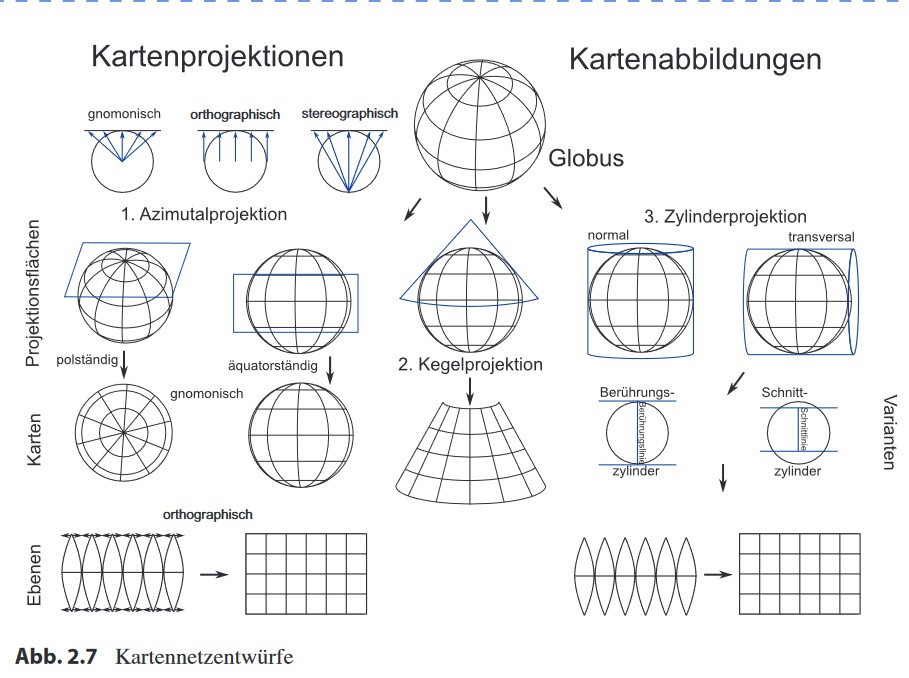
\includegraphics[width=\linewidth]{images/Kartennetzentwurfe.jpg}
%   \caption{Kartennetzentwürfe}
%   \label{fig:meineabbildung}
% \end{figure}

% Das geodätische Lagekoordinationssystem bezieht sich auf das System zur Bestimmung der genauen Position von Objekten auf der Erdoberfläche, während eine Projektion die Methode ist, wie diese Position auf eine Karte dargestellt wird.\\



% Geodaten unterscheiden sich in Geobasis- und Geofachdaten.
% Geobasisdaten sind von den amtlichen Vermessungseinrichtungen in einem einheitlichen geodätischen Bezugssystem bereitgestellten topographischen Daten, die die wesentlichen Objekte der Erdoberfläche (Siedlungen, Verkehrsnetze, Vegetation, Gewässer, Geländeformen und Grenzen politischer und administrativer Einheiten) anwendungsneutral beschreiben. Alle erfassten Geobasisdaten werden in digitaler Form im Topographisch-Kartographischen Informationssystem bei den Vermessungsverwaltungen der Länder vorgehalten. (adv-online.de geodatenzentrum.de). Geobasisdaten bilden topographische „Grundgerüst“.

% Geofachdaten sind raumbezogene thematische Daten, die fachgebietsbezogen erfasst und bereitgestellt werden und sich auf alle Gegenstände und Sachverhalte mit geographischem Bezug erstrecken können. Beispiele seien Wetter- und Klimadaten, Daten zum Umweltzustand, Landnutzungsdaten und statische Daten.

% Kartennetzentwürfe sind zweidimensionale Kartendarstellungen der gekrümmten Erdoberfläche.\\

% \begin{figure}[ht]
%   \centering
%   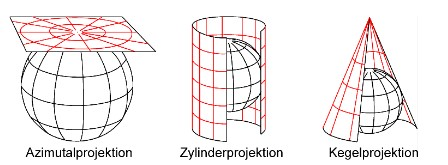
\includegraphics[width=\linewidth]{images/kartennetz.jpg}
%   \caption{Klassifikation der Kartennetzentwürfe nach der Art der Abbildungsflächen}
%   \label{fig:meineabbildung}
% \end{figure}